\chapter{Lecture 1}

\section{History}

\begin{center}
  \begin{tabular}{ccccc}
    Date & People & What & Why & Techniques \\
    \midrule
    1969 &
    \makecell{ Faddeev \\ and Popov } &
    \makecell{ Gauge fixing \\ (adding ghosts) } &
    \makecell{ Quantize \\ Yang-Mills } &
    \makecell{ Berezinian \\ integration } \\
    \addlinespace
    1973 & 
    \makecell{ 't Hooft and \\ Veltman } &
    \makecell{ Quantized \\ Yang-Mills } &
    \makecell{ Quantize \\ Yang-Mills } &
    \makecell{ Feynman \\ diagrams } \\
    \addlinespace
    1975 &
    \makecell{ Becchi, Rouet, \\ Stora, Tyutin \\ (BRST) } &
    \makecell{ Cohomological \\ theory to quantize \\ Yang-Mills } &
    \makecell{ Understanding \\ 't Hooft \\ and Veltman } &
    \makecell{ Derived invariants \\ (Lie algebra \\ cohomology) } \\
    \addlinespace
    1981 &
    \makecell{ Batallin and \\ Vilkovisky \\ (BV) } &
    \makecell{ Quantize systems \\ with complicated \\ gauge symmetries } &
    Supergravity &
    \makecell{ Derived \\ intersections \\ (Koszul complexes) } \\
    \addlinespace
    1992 & Henneaux &
    \makecell{ Quantize \\ Yang-Mills \\ using BV } &
    \makecell{ Analyze \\ Yang-Mills \\ using BV } &
    \makecell{ Derived \\ intersections} \\
    \addlinespace
    2007 & Costello &
    \makecell{ Combine BV \\ with effective \\ field theory } &
    \makecell{ Make BV \\ quantization \\ rigorous } &
    \makecell{ Derived everything, \\ analysis, and \\ homotopy theory }
  \end{tabular}
\end{center}

\section{References}

The main references for this seminar will be:

\begin{itemize}
  \item Costello - Renormalization and Effective Field Theory \cite{costelloRenormalizationEffective};
  \item Elliot, Williams, Yoo - Asymptotic Freedom in the BV Formalism \cite{elliottAsymptoticFreedom};
  \item Gwilliam - Factorization algebras and free field theories \cite{gwilliamFactorizationAlgebras}.
\end{itemize}

\section{Roadmap to BV Quantization}

\begin{figure}
  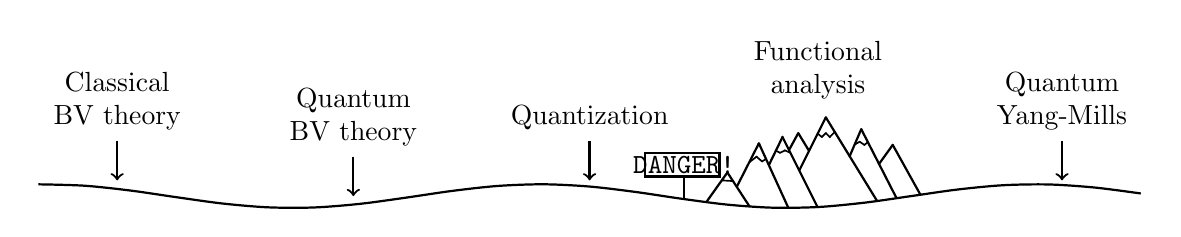
\begin{tikzpicture}
  \draw[thick, domain=-7:7, smooth, variable=\x] plot ( {\x}, {0.15*sin(deg(\x+2.2))} );
  \node at (-6, 1.2) {
    \begin{tabular}{c}
      Classical \\
      BV theory
    \end{tabular}
  };
  \draw[thick, ->] (-6, .7) -- (-6, .2);
  \node at (-3, 1) {
    \begin{tabular}{c}
      Quantum \\
      BV theory
    \end{tabular}
  };
  \draw[thick, ->] (-3, .5) -- (-3, 0);
  \node at (0, 1) { Quantization };
  \draw[thick, ->] (0, .7) -- (0, .2);
  \node at (2.9, 1.6) {
    \begin{tabular}{c}
      Functional \\
      analysis
    \end{tabular}
  };
  \node at (1.2, .4) { \miniscule\texttt{DANGER!} };
  \draw[thick] (.7, .25) rectangle ++(.95, .3);
  \draw[thick] (1.2, .25) -- (1.2, -.03);
  \node at (6, 1.2) {
    \begin{tabular}{c}
      Quantum \\ 
      Yang-Mills
    \end{tabular}
  };
  \draw[thick, ->] (6, .7) -- (6, .2);
  % Mountains
  \draw[thick] (1.48, -.08) -- (1.75, 0.3);
  \draw[thick] (1.75, 0.3) -- (2.03, -.13);
  \draw[fill] (1.75, 0.3) circle (.2pt);
  \draw[semithick] (1.67, .2) -- (1.83, 0.19);
  \draw[thick] (1.87, .12) -- (2.15, 0.67);
  \draw[thick] (2.15, 0.67) -- (2.52, -.14);
  \draw[fill] (2.15, 0.67) circle (.19pt);
  \draw[semithick] (2.03, 0.43) -- (2.12, 0.5);
  \draw[fill] (2.12, 0.5) circle (.101pt);
  \draw[semithick] (2.12, 0.5) -- (2.19, 0.44);
  \draw[fill] (2.19, 0.44) circle (.101pt);
  \draw[semithick] (2.19, 0.44) -- (2.24, 0.47);
  \draw[thick] (2.28, .4) -- (2.45, 0.75);
  \draw[thick] (2.45, 0.75) -- (2.9, -.15);
  \draw[fill] (2.45, 0.75) circle (.19pt);
  \draw[semithick] (2.36, 0.58) -- (2.42, 0.55);
  \draw[fill] (2.42, 0.55) circle (.101pt);
  \draw[semithick] (2.42, 0.55) -- (2.48, 0.58);
  \draw[fill] (2.48, 0.58) circle (.101pt);
  \draw[semithick] (2.48, 0.58) -- (2.55, 0.55);
  \draw[thick] (2.53, .58) -- (2.65, 0.8);
  \draw[thick] (2.65, 0.8) -- (2.79, .57);
  \draw[fill] (2.65, 0.8) circle (.19pt);
  \draw[thick] (2.66, .32) -- (3, 1);
  \draw[thick] (3.65, -.06) -- (3, 1);
  \draw[fill] (3, 1) circle (.19pt);
  \draw[semithick] (2.89, .8) -- (2.95, .75);
  \draw[fill] (2.95, 0.75) circle (.101pt);
  \draw[semithick] (2.95, .75) -- (3, .8);
  \draw[fill] (3, 0.8) circle (.101pt);
  \draw[semithick] (3, .8) -- (3.05, 0.75);
  \draw[fill] (3.05, 0.75) circle (.101pt);
  \draw[semithick] (3.05, 0.75) -- (3.12, 0.82);
  \draw[thick] (3.3, 0.5) -- (3.45, 0.85);
  \draw[thick] (3.45, 0.85) -- (3.9, -.03);
  \draw[fill] (3.45, 0.85) circle (0.19pt);
  \draw[semithick] (3.36, .65) -- (3.43, .69);
  \draw[fill] (3.43, .69) circle (.101pt);
  \draw[semithick] (3.43, .69) -- (3.49, .65);
  \draw[fill] (3.49, .65) circle (.101pt);
  \draw[semithick] (3.49, .65) -- (3.54, .69);
  \draw[thick] (3.67, .4) -- (3.85, .65);
  \draw[thick] (3.85, 0.65) -- (4.2, 0.02);
  \draw[fill] (3.85, 0.65) circle (.19pt);
\end{tikzpicture}
\centering
\caption{Roadmap to BV quantization.}
\label{fig:roadmap}
\end{figure}

The space of fields $\Ecal^\bullet$ is a cochain complex
\begin{equation*}
  \begin{tikzcd}
    \dots \arrow[r] &
    \Ecal^{-1} \arrow[r, "Q"] &
    \Ecal^0 \arrow[r, "Q"] &
    \Ecal^1 \arrow[r, "Q"] &
    \Ecal^2 \arrow[r] &
    \dots
  \end{tikzcd}
\end{equation*}
equipped with a differential $Q$ such that $Q^2 = 0$. Moreover, $\Ecal$ admits a $-1$-shifted symplectic structure, that is, there exists a non degenerate pairing of degree $-1$
\begin{equation*}
  \langle \cdot , \cdot \rangle :
  \Ecal \otimes \Ecal \longrightarrow \Rbb [-1]
\end{equation*}
such that $\langle x, y \rangle = -(-1)^{(|x|+1)(|y|+1)} \langle y, x \rangle$. This structure defines a $+1$-shifted Poisson bracket
\begin{equation*}
  \{ \cdot, \cdot \} :
  \Ocal( \Ecal ) \otimes \Ocal( \Ecal ) \longrightarrow \Ocal( \Ecal )
\end{equation*}
where $\Ocal ( \Ecal ) \cong \mathrm{Sym}^\bullet (\Ecal^\vee)$ is the (graded) commutative algebra of polynomial functions on the dual complex $\Ecal^\vee$. Pick $S \in \Ocal (\Ecal)$ obeying the \textbf{classical master equation} (CME)
\begin{equation}
  \label{eq:cme}
  \{ S, S \} = 0.
\end{equation}
The data $(\Ecal, \langle \cdot, \cdot \rangle, S)$ defines a \textbf{classical BV theory}. The CME says $\{ S, \cdot \}$ is a differential which makes $(\Ocal ( \Ecal ), \{S, \cdot \} )$ into a cochain complex such that
\begin{equation*}
  \Hrm^0 \Ocal ( \Ecal ) \cong
  \Ocal( \mathrm{Crit} (S) ),
\end{equation*}
where $\mathrm{Crit} (S)$ denotes the critical locus of $S$. We will restrict to $S$ of the form
\begin{equation*}
S(e) = \underbrace{\langle e, Qe \rangle}_{\substack{ \text{free part} \\ \text{(kinetic +} \\ \text{mass terms)} }}
+ \underbrace{I(e)}_{\substack{ \text{interaction} \\ \text{part (cubic} \\ \text{or higher)} }}.
\end{equation*}

\begin{example}
  Why are the cubic and higher order terms called interaction terms? For electromagnetism on a manifold $M$ we have a space of fields
  $\Fcal = \Omega^1(M) \oplus \Omega^0(M, S)$ in degree $0$. Let $F = \drm A$ and define
  \begin{equation*}
    S(A, \psi) = \int_M
    \underbrace{F \wedge \hodge F
    + \langle \psi, \slashed{\drm} \psi \rangle \dd \mathrm{vol}}_{\text{quadratic terms}}
    + \underbrace{\langle \psi, \slashed{A} \psi \rangle \dd \mathrm{vol}}_{\text{interaction term}}.
  \end{equation*}
  Computing the Euler-Lagrange equations we obtain the system of differential equations
  \begin{equation*}
    \begin{cases}
      \hodge \drm \hodge F = \bar{\psi} \gamma^\mu \psi \dd x_\mu \\
      \slashed{d}_A \psi = 0
    \end{cases}
  \end{equation*}
  which is coupled because of the interaction term.
\end{example}

\section{Quantization in the BV formalism}

The slogan of quantization in the BV formalism is to \emph{deform the differential}. In the perturbative context we work in formal power series in $\hbar$, for example, over the ring $\Rbb[[\hbar]]$. Quantization results in a cochain complex
$(\Ocal(\Ecal)[[\hbar]], \{S^q, \cdot\} + \hbar \Delta)$, where $\Delta$ is called the BV Laplacian, and 
$S^q \in \Ocal(\Ecal)[[\hbar]]$ satisfies the \textbf{quantum master equation} (QME)
\begin{equation}
  \label{eq:qme}
  (\{S^q, \cdot \} + \hbar \Delta)^2 = 0
\end{equation}

\begin{example}
  In finite dimensions ($\Fcal \cong \Rbb^n$) the BV fields are
  $\Ecal = \Rbb^n \longrightarrow \Rbb^n$
  therefore
  \begin{equation*}
    \Ocal(\Ecal) \cong \Rbb [x^1, \dots, x^n, \xi^1, \dots, \xi^n]
  \end{equation*}
  and the BV Laplacian takes the form
  \begin{equation*}
    \Delta = \sum_{\mu = 1}^n \frac{\partial}{\partial \xi^\mu} \frac{\partial}{\partial x^\mu}.
  \end{equation*}
  In this form, it becomes clear that $\Delta$ is a differential operator of degree $1$ such that $\Delta^2 = 0$.
\end{example}
\begin{equation*}
  S^q(e) = \langle e, Qe \rangle
  + I^q(e)
\end{equation*}
where $I^q \in \Ocal(\Ecal) [[\hbar]]$ is cubic mod $\hbar$ and satisfies the QME
\begin{equation*}
  Q I^q + \frac{1}{2} \{I^q, I^q\} + \hbar \Delta I^q = 0
\end{equation*}
which resembles, in this form, the \textbf{Maurer-Cartan} (MC) \textbf{equation}. In infinite dimensions, some problems arise:

\begin{enumerate}
  \item there may be no solution to this equation. In this case we say that quantization is obstructed (there is an anomaly);
  \item the QME in infinite dimensions is ill-defined. Some functional analysis is needed to make sense of this problem.
\end{enumerate}
